\chapter{Perintah-perintah dasar}


\section{Penggunaan Sitasi}
Contoh penggunaan sitasi \cite{lukito2016,santosa2011user}
\cite{setiawan2014fuzzy} \cite{wibowo2014line} \cite{marenda2016digitory} \cite{wibirama2013dual,wibowo2016clustering}

\section{Penulisan Gambar}

\begin{figure}[h]
	\centering
	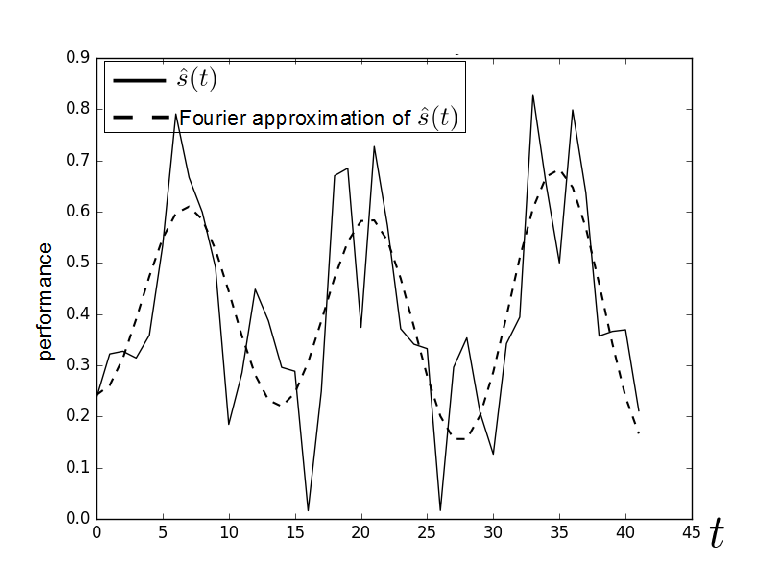
\includegraphics[width=10cm]{images/sample-fig.png}
	\caption{Contoh gambar.}
	\label{Fig: Contoh gambar}
\end{figure}

Contoh gambar terlihat pada Gambar \ref{Fig: Contoh gambar}. Gambar diambil dari \cite{wibowo2016clustering}.

\section{Penulisan Tabel}
\begin{table}[h]
	\caption{tabel ini}
	\vspace{0.5em}
	\centering
	\begin{tabular}{|l|r|r|}
		\hline
		ID & Tinggi Badan (cm) & Berat Badan (kg) \\
		\hline \hline
		A23 & 173 & 62 \\
		A25 & 185 & 78 \\
		A10 & 162 & 70 \\ \hline
	\end{tabular}
	\label{Tab: Tabel Tinggi Berat}
\end{table}

Contoh penulisan tabel bisa dilihat pada Tabel \ref{Tab: Tabel Tinggi Berat}.

\begin{table}[h]
	\caption{tabel ini}
	\vspace{0.5em}
	\centering
	\begin{tabulary}{\linewidth}{|l|C|C|}
		\hline
		ID & Tinggi Badan Mahasiswa di Universitas Gadjah Mada (cm) & Berat Badan Mahasiswa di Universitas Gadjah Mada(kg) \\
		\hline \hline
		A23 &  \multicolumn{1}{r|}{173} &  \multicolumn{1}{r|}{62} \\
		A25 &  \multicolumn{1}{r|}{185} &  \multicolumn{1}{r|}{78} \\
		A10 &  \multicolumn{1}{r|}{162} &  \multicolumn{1}{r|}{70} \\ \hline
	\end{tabulary}
	\label{Tab: Tabel Tinggi Berat Kolom Panjang}
\end{table}

Contoh penulisan tabel dengan nama kolom sangat panjang denagn bantuan \textit{tabulary} bisa dilihat pada Tabel \ref{Tab: Tabel Tinggi Berat Kolom Panjang}.

\section{Penulisan formula}
Contoh penulisan formula
\begin{equation}
L_{\psi_z} = \{ t_i \mid v_z(t_i) \le \psi_z \}
\end{equation}

Contoh penulisan secara \textit{inline}: $\mathit{PV = nRT}$. Untuk kasus-kasus tertentu, kita membutuhkan perintah "mathit" dalam penulisan formula untuk menghindari adanya jeda saat penulisan formula.

Contoh formula \textbf{tanpa} menggunakan "mathit": $PVA = RTD$

Contoh formula \textbf{dengan} menggunakan "mathit": $\mathit{PVA = RTD}$

Untuk mengutip persamaan dapat juga menggunakan (\ref{eq:miqp-obj}). Persamaan dapat ditulis secara sentral pada file "equations/equations.tex".
    
    \inputeq{equations/equations}{miqp-obj}


\section{Contoh list}
Berikut contoh penggunaan list
\begin{enumerate}
	\item First item
	\item Second item
	\item Third item
\end{enumerate}

\section{Contoh \textit{highlight}}
Berikut contoh penggunaan \hly{\textit{highlight} kuning menggunakan} \verb|\hly{}|. Pengunaan \textit{highlight} tidak disarankan untuk dua paragraf sekaligus karena dapat mengakibatkan kerusakan dalam penomoran.

\hly{Gunakan perintah} \verb|\hly{}| yang terpisah untuk tiap paragrafnya seperti ini.

\hly{Penggunaan tanda \textit{curly bracket} \{ \} di dalam \textit{highlight} seperti penggunaan} \verb|\textit{}| \hlr{diperbolehkan, namun penghapusan otomatis oleh} \verb|"utilities/remove_highlight.ipynb"| \hly{tidak mendukung penghapusan \textit{nested bracket} seperti itu. Alternatifnya gunakan pemisahan} \textit{for the italic text} \hlg{seperti ini.}
